\newpage
\question ~\\
\begin{center}
        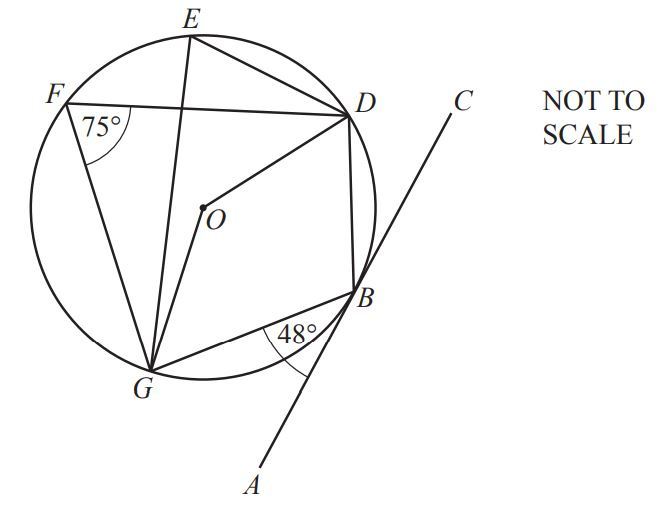
\includegraphics[scale=0.6]{Questions/quiz 19/images/9.JPG}
\end{center} 
$B, D, E, F$ and $G$ are points on the circumference of a circle centre $O$.\\
$A C$ is a tangent to the circle at $B$.\\
Angle $D F G=75^{\circ}$ and angle $A B G=48^{\circ}$.\\
\begin{parts}
\part 
Find angle $D E G$.\\ \\
{\flushright{
\hfill      Angle $D E G=$    \makebox[12em]{\dotfill}  [1]}}
\\ \\
\part Find angle $D OG$.\\ \\
{\flushright{
\hfill         Angle $D OG$ \makebox[12em]{\dotfill}  [1]}}\\ 
\part Find angle $DBC$.\\ \\
{\flushright{
\hfill         Angle $D BC$ \makebox[12em]{\dotfill}  [2]}}
\end{parts}